\section{Density Stratified Flow}
For a velocity profile the same as in \eqref{kh:bg}
\begin{equation*}
\mathbf{U}(z) =
\begin{cases} U_0 \mathbf{i} &\text{if $z>0$,}\\
-U_0 \mathbf{i} &\text{if $z<0$.}
\end{cases}
\end{equation*}
with the boundary conditions $\phi \to 0$ as $z \to \pm\infty$,
$c=c_R+ic_I$ is complex in general. But the density is stratified by
a constant $N^2\equiv-(g/\rho_0)(d\rho/dz)$. The Boussinesq
approximation is applied so that the variation in density only
appears in the buoyancy term.

Taylor-Goldstein equation \eqref{tay:eq2} is required to solve this
problem. By matching the boundary conditions at $z=0$ in general
case of \eqref{kh:pro}, I found $c_R=(U_1+U_2)/2$, which is
\begin{equation}\label{str:cr}
    c_R=\frac{U_0-U_0}{2}=0
\end{equation}
We have two types of solutions:
\begin{enumerate}
\item[(A)] Neutral Solutions: $c_I=0$

For $\alpha^2>N^2/U^2$, the trial solution is
\begin{equation}\label{str:tr1}
\phi =
\begin{cases}
Ae^{-nz} &\text{if $z>0$,}\\
Be^{nz} &\text{if $z<0$.}
\end{cases}
\qquad \text{where }n=\sqrt{\alpha^2-\frac{N^2}{U^2}}
\end{equation}
Matching boundary conditions at $z=0$:
\begin{enumerate}
  \item[(i)] pressure: $-nU_0A=n(-U_0)B \quad\Rightarrow A=B$
  \item[(ii)] displacement: $A/U_0=B/{-U_0} \quad\Rightarrow A={-B}$
\end{enumerate}
Therefore $A=B=0$. There is no neutral solution for
$\alpha^2>N^2/U^2$.

For $\alpha^2<N^2/U^2$, the trial solution is
\begin{equation}\label{str:tr2}
\phi =
\begin{cases}
Ae^{inz} &\text{if $z>0$,}\\
Be^{inz} &\text{if $z<0$.}
\end{cases}
\qquad \text{where }n=\pm\sqrt{\frac{N^2}{U^2}-\alpha^2}
\end{equation}
Matching boundary conditions at $z=0$:
\begin{enumerate}
  \item[(i)] pressure: $-inU_0A=-in(-U_0)B \quad\Rightarrow A={-B}$
  \item[(ii)] displacement: $A/U_0=B/{-U_0} \quad\Rightarrow A={-B}$
\end{enumerate}
To satisfy the radiative boundary conditions at $z \to \pm\infty$,
we have the vertical components of the energy flux
as\footnote{$\langle\quad\rangle$ means average value.}
\begin{align}
    \langle F_z\rangle&=\langle\text{Re}(p')\text{Re}(w')\rangle\notag\\
    &=\langle\text{Re}(-inU\phi e^{i(\alpha x-\alpha c t)})\text{Re}(-i\alpha\phi e^{i(\alpha x-\alpha c t)})\rangle\notag\\
    &=\frac{1}{2}\text{Re}(nU\alpha\phi^*e^{-i(\alpha x-\alpha c t)}\phi e^{i(\alpha x-\alpha c t)})\notag\\
    &=\frac{1}{2}\text{Re}(nU\alpha\phi^*\phi)\notag\\
    &=\frac{1}{2}nU\alpha\lvert A\rvert^2\label{str:rad}
\end{align}
For $z>0$,
\begin{equation*}
    U=U_0,\quad\langle F_z\rangle>0 \quad\Rightarrow n>0
\end{equation*}
For $z<0$,
\begin{equation*}
    U=-U_0,\quad\langle F_z\rangle<0 \quad\Rightarrow n>0
\end{equation*}
Therefore the natural solution is
\begin{equation}\label{str:sol1}
\phi =
\begin{cases}
Ae^{inz} &\text{if $z>0$,}\\
-Ae^{inz} &\text{if $z<0$.}
\end{cases}
\qquad \text{where }n=\sqrt{\frac{N^2}{{U_0}^2}-\alpha^2},\quad
\alpha^2<\frac{N^2}{{U_0}^2}
\end{equation}
\begin{equation}\label{str:c1}
    \boxed{c=0,\qquad\alpha^2<\frac{N^2}{{U_0}^2}}
\end{equation}
\item[(B)] Unstable Solutions: $c_I\neq0$

The trial solution is
\begin{equation}\label{str:tr3}
\phi =
\begin{cases}
Ae^{-nz} &\text{if $z>0$,}\\
Be^{n^*z} &\text{if $z<0$.}
\end{cases}
\qquad \text{where }n^2=\alpha^2-\frac{N^2}{(U-ic_I)^2}
\end{equation}
$n$ is chosen to have positive real part so that the solution
vanishes when $z \to \pm\infty$. When $\text{Re}(n)=0$,
$\text{Im}(n)<0$ which automatically satisfied the radiative
boundary conditions as shown in \eqref{str:rad}.

Matching boundary conditions at $z=0$:
\begin{enumerate}
  \item[(i)] pressure: $n(U_0-ic_I)A=n^*(U_0+ic_I)B$
  \item[(ii)] displacement: $A/(U_0-ic_I)=B/({-U_0}-ic_I)$
\end{enumerate}
Combining the two equations to get
\begin{equation}\label{str:b1}
    n(U_0-ic_I)^2=-n^*(U_0+ic_I)^2
\end{equation}
Which can be written as $n(U_0-ic_I)^2 = -(n(U_0-ic_I)^2)^*$,
therefore I have
\begin{equation}
    \text{Re}\Bigl(n(U_0-ic_I)^2\Bigr)=0\label{str:b2}
\end{equation}
Then expand $n(U_0-ic_I)^2$ as
\begin{equation}
    n(U_0-ic_I)^2=({U_0}^2-2iU_0c_I-{c_I}^2)(n_R+in_I)\label{str:b3}
\end{equation}
By comparing real part of \eqref{str:b2} and \eqref{str:b3},
\begin{equation}
    n_R=-\frac{2c_IU_0}{{U_0}^2-{c_I}^2}n_I\label{str:b4}
\end{equation}
Write $n$ as
$n=n_R+in_I=\Bigl(-\frac{2c_IU_0}{{U_0}^2-{c_I}^2}+1\Bigr)n_I$, take
square and compare the real and imaginary parts with the definition
in \eqref{str:tr3}, I get
\begin{align}
    {c_I}^2 &={U_0}^2-\frac{N^2}{2\alpha^2},\qquad\text{where }\alpha^2>\frac{N^2}{2{U_0}^2}\label{str:sol1}\\
    n^2 &=-\alpha^2\frac{(U+ic_I)^2}{(U-ic_I)^2}\label{str:sol2}
\end{align}
$c$ is found to be:
\begin{equation}\label{str:c2}
    \boxed{c=\pm
    i\sqrt{{U_0}^2-\frac{N^2}{2\alpha^2}},\qquad\alpha^2>\frac{N^2}{2{U_0}^2}}
\end{equation}
\end{enumerate}
The unstable solution is plotted in Figure \ref{kh2}. The density
stratification tends to stabilize long waves with smaller wave
number $\alpha$.
\begin{figure}[htpb]
  \centering
  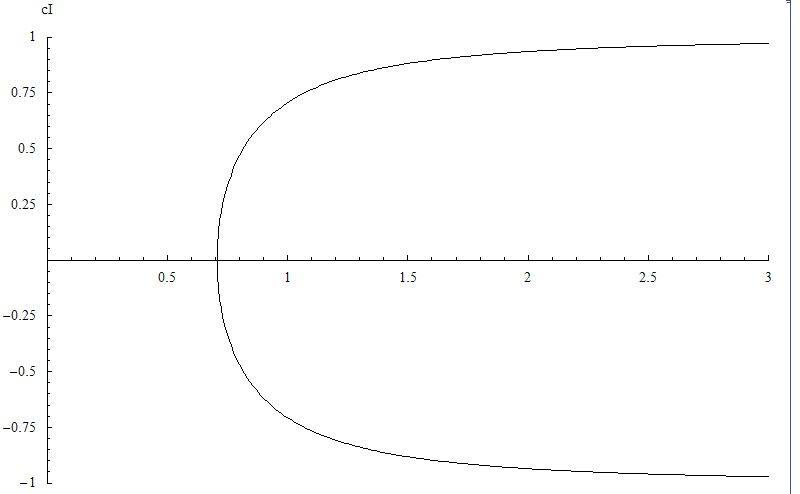
\includegraphics[width=0.9\textwidth]{kh2.png}\\
  \caption{$c_I$ vs.~$\alpha$ for $U_0=1$ of a stratified KH mode}\label{kh2}
\end{figure}
